\section{图像外观}
\label{sec:plot-appearance}

\subsection{图像元素}
对于SAC而言,最基本的显示元素是将所有数据点用线连起来所构成的地震图。
除此之外,SAC的绘图命令还会在图像的四个边绘制坐标轴以及刻度,为图像
添加标题、轴标签等。

图 \ref{fig:plot-appearance} 展示了一个完整的SAC图像所包含的所有元素。

\begin{figure}[H]
\centering
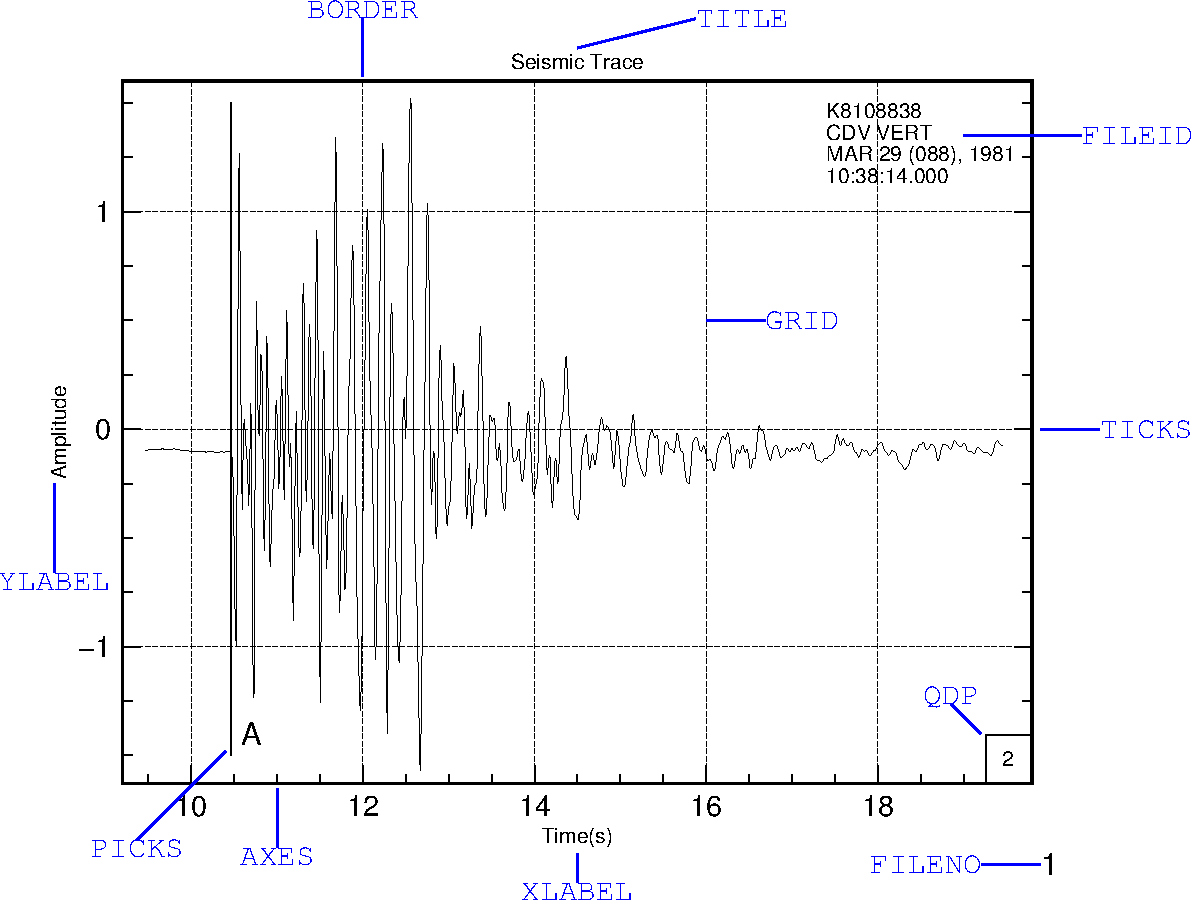
\includegraphics[width=0.9\textwidth]{appearance}
\caption[绘图外观相关命令]{绘图外观及其相关命令。图中蓝色部分为对
    绘图外观的说明。}
\label{fig:plot-appearance}
\end{figure}

图 \ref{fig:plot-appearance} 可以用如下命令绘制得到:
\begin{SACCode}
SAC> fg seis                // 生成数据
SAC> qdp on                 // 打开QDP选项(默认值即为开)
SAC> grid on                // 显示网格
SAC> title 'Seismic Trace'  // 设置标题
SAC> xlabel "Time(s)"       // 设置x轴标签
SAC> ylabel "Amplitude"     // 设置y轴标签
SAC> filenumber on          // 显示文件号
SAC> axes only left bottom  // left和bottom显示axes
SAC> ticks only right       // right显示ticks
SAC> border on              // top显示border
SAC> p                      // 绘图
\end{SACCode}

图像中显示的元素包括:
\subsubsection{标签}
标签大致可以分为三种:标题、轴标签和通用标签。
\begin{description}
\item[TITLE] 图像的标题。\nameref{cmd:title} 命令可控制标题文本、位置和尺寸
\item[XLABEL、YLABEL] 轴标签。\nameref{cmd:xlabel} 和 \nameref{cmd:ylabel}
    命令可指定X和Y轴标签文本、位置和尺寸。
\item[PLABEL] 通用标签。\nameref{cmd:plabel} 可指定通用标签的文本、位置和尺寸。
\end{description}

标签文本需要用单引号或双引号包围,文本尺寸选项 !size! 可以选择
!tiny!、!small!、!medium! 或 !large!,
文本位置选项 !location! 则可以取 !top!、!bottom!、
!left! 或 !right!。

可以通过 \nameref{cmd:plabel} 命令定义最多三个通用标签。通用标签与轴标
签类似,其更通用之处在于可以任意指定其位置。每个标签可以用
!position x y a! 来指定其位置,其中x、y为标签位置相对于窗口尺寸
的比例,a表示标签相对于水平方向顺时针旋转的角度;也可以用 !below!
设置新标签位于上一标签的下方。

\subsubsection{标记}
图像中包含了如下标记:
\begin{description}
\item [FILEID] 文件ID。\nameref{cmd:fileid} 用于控制文件ID的内容、位置及其格式。
\item [FILENO] 文件号。\nameref{cmd:filenumber} 控制文件号显示与否。
\item [PICKS] 到时标记。\nameref{cmd:picks} 用于控制是否显示到时标记以及显示效果。
\item [QDP] QDP因子。\nameref{cmd:qdp} 用于控制qdp因子的大小。
\end{description}

QDP,全称为``quick and dirty plot''。在开发SAC的那个年代,计算机的性能
一般,若在绘图时绘制全部数据点,则绘图过程会耗费大量时间。因而SAC采用了
``qdp''的方式:每隔若干个数据点绘制一个数据点\footnote{本质上就是绘图时
的一次``减采样'',但是没有做抗混淆处理。}。图中右下角的``2''即表示每两个
点中绘制一个点。目前计算机的性能已经足够强大,因而一般使用 !qdp off!
命令关闭该选项。

\subsubsection{框架}
每张图都有一个框架,每个框架有TOP、BOTTOM、LEFT和RIGHT四条边。

SAC中,每条边都可以用四种不同的形式表示:
\begin{itemize}
\item 不绘制;
\item border:仅一条直线,即图 \ref{fig:plot-appearance} 中TOP边;
\item ticks:直线+刻度\footnote{刻度专指每条边上的短线。},即图中RIGHT边;
\item axes:直线+刻度+标注\footnote{标注专指每条边上的数字。},
    即图中LEFT边和BOTTOM边;
\end{itemize}

从上面的定义可以看到,四种形式的边存在包含与被包含的关系,因而在设
定边时,有如下规则:
\begin{enumerate}
\item 用 \nameref{cmd:axes} 控制在哪些边使用``axes'';
\item 只有不使用``axes''的边才可以用 \nameref{cmd:ticks} 命令控制
    是否使用``ticks'';
\item 只有不使用``axes''和``ticks''的边才可以使用 \nameref{cmd:border}
    命令控制是否使用``border'';
\item 不使用``axes''、``ticks''和``borders''的边则不绘制。
\end{enumerate}

除了边之外,还可以使用 \nameref{cmd:grid} 命令控制网格的显示以及网格的
线型,或使用 \nameref{cmd:xgrid}、\nameref{cmd:ygrid} 分别控制横、纵方
向网格的显示和属性。

\subsection{图像控制}
\subsubsection{坐标轴}
SAC使用了优秀的默认算法,根据要绘制的数据范围选择合适的刻度间隔和标注。
若对于默认的结果不满意,可以使用SAC提供的命令分别对X、Y坐标轴进行调整,
下面仅列出与X轴相关的命令。
\begin{description}
\item [xlim] 控制绘图的X轴范围
\item [xdiv] 控制X轴刻度间隔
\item [xfudge] 设定fudge因子,根据数据极值扩展X轴范围
\end{description}

\subsubsection{坐标系}
绘制时间序列一般使用线性坐标系,SAC也提供了一系列命令以指定X、Y轴为线性
坐标轴或对数坐标轴。这些命令包括: \nameref{cmd:linlin}、\nameref{cmd:linlog}、
\nameref{cmd:loglin}、\nameref{cmd:loglog}、\nameref{cmd:xlin}、\nameref{cmd:xlog}、
\nameref{cmd:ylin}、\nameref{cmd:ylog}。

对于对数坐标轴,还有一些命令可以控制其外观,比如 \nameref{cmd:xfull}、
\nameref{cmd:loglab}、\nameref{cmd:floor}。

\subsection{线条属性}
\label{subsec:line-attribution}

线条的属性包括线型(\nameref{cmd:line})、线宽(\nameref{cmd:width})、
颜色(\nameref{cmd:color})和符号(\nameref{cmd:symbol})。

下面的命令展示了如何修改线条的属性。
\begin{SACCode}
SAC> fg seis
SAC> line 3         // 线型为3
SAC> width 2        // 线宽为2
SAC> color red      // 红色
SAC> p
\end{SACCode}

\begin{figure}[H]
\centering
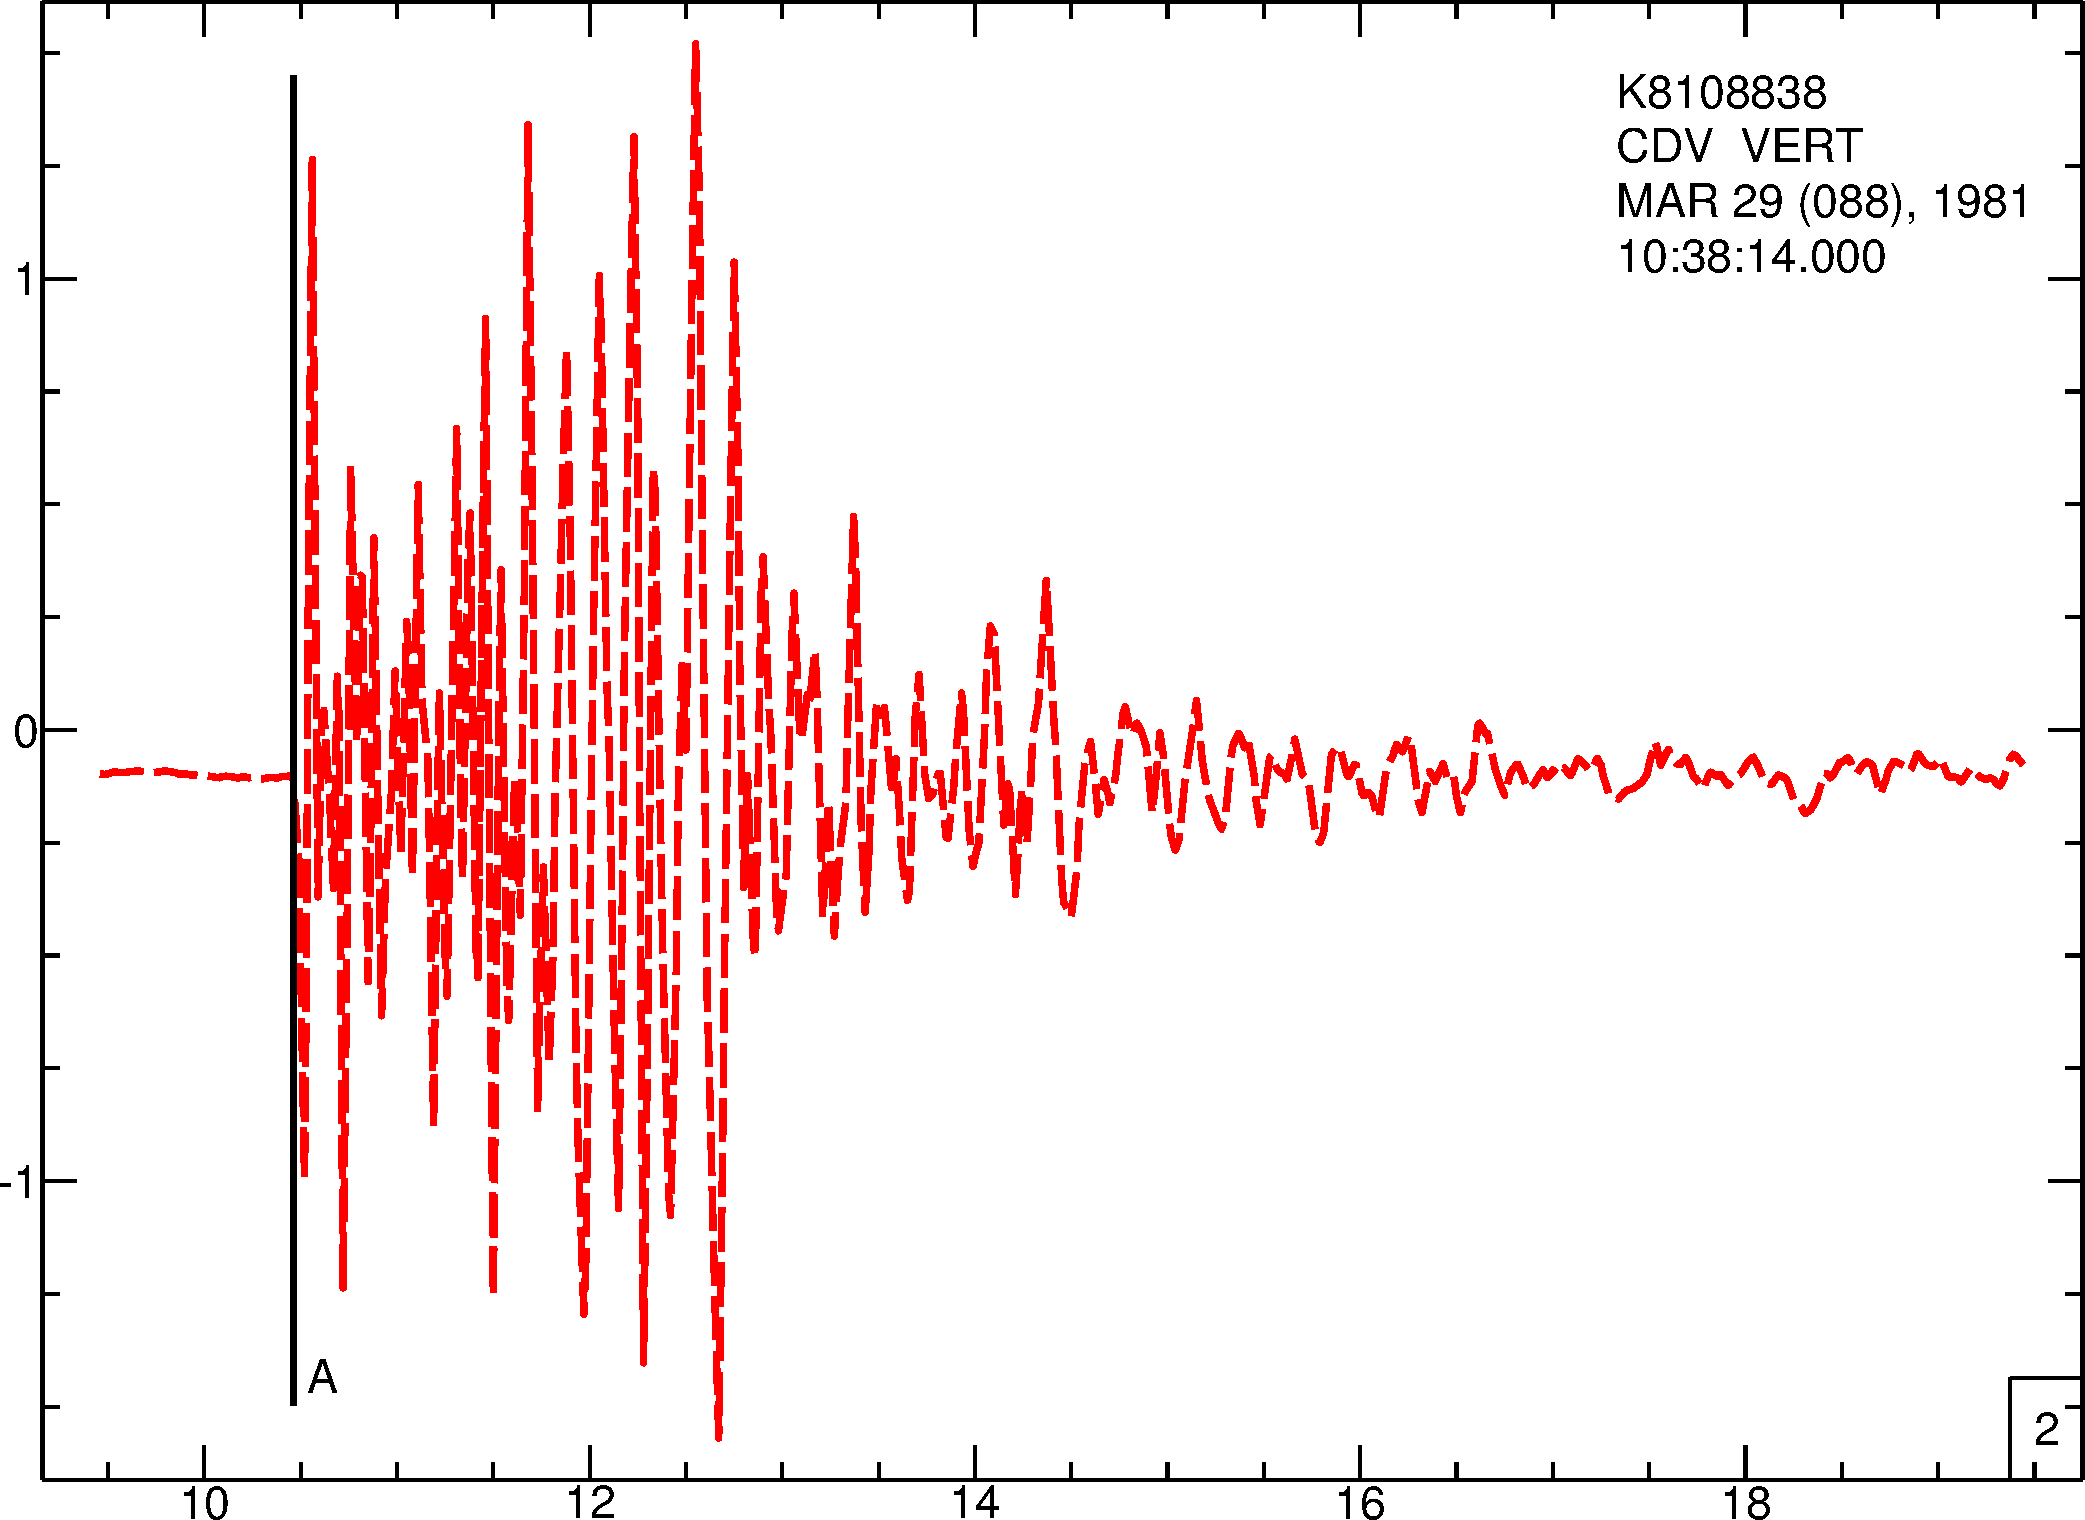
\includegraphics[width=0.7\textwidth]{attribution1}
\caption{线条属性}
\end{figure}

在绘制多个波形数据时,可以设置线条的属性按照某个列表递增。下面的命令
一次绘制四个波形文件,使每个数据的线型和颜色都按照默认列表递增。
\begin{SACCode}
SAC> dg sub teleseis ntkl.z nykl.z onkl.z sdkl.z
SAC> line incre
SAC> color black incre
SAC> p
\end{SACCode}

\begin{figure}[H]
\centering
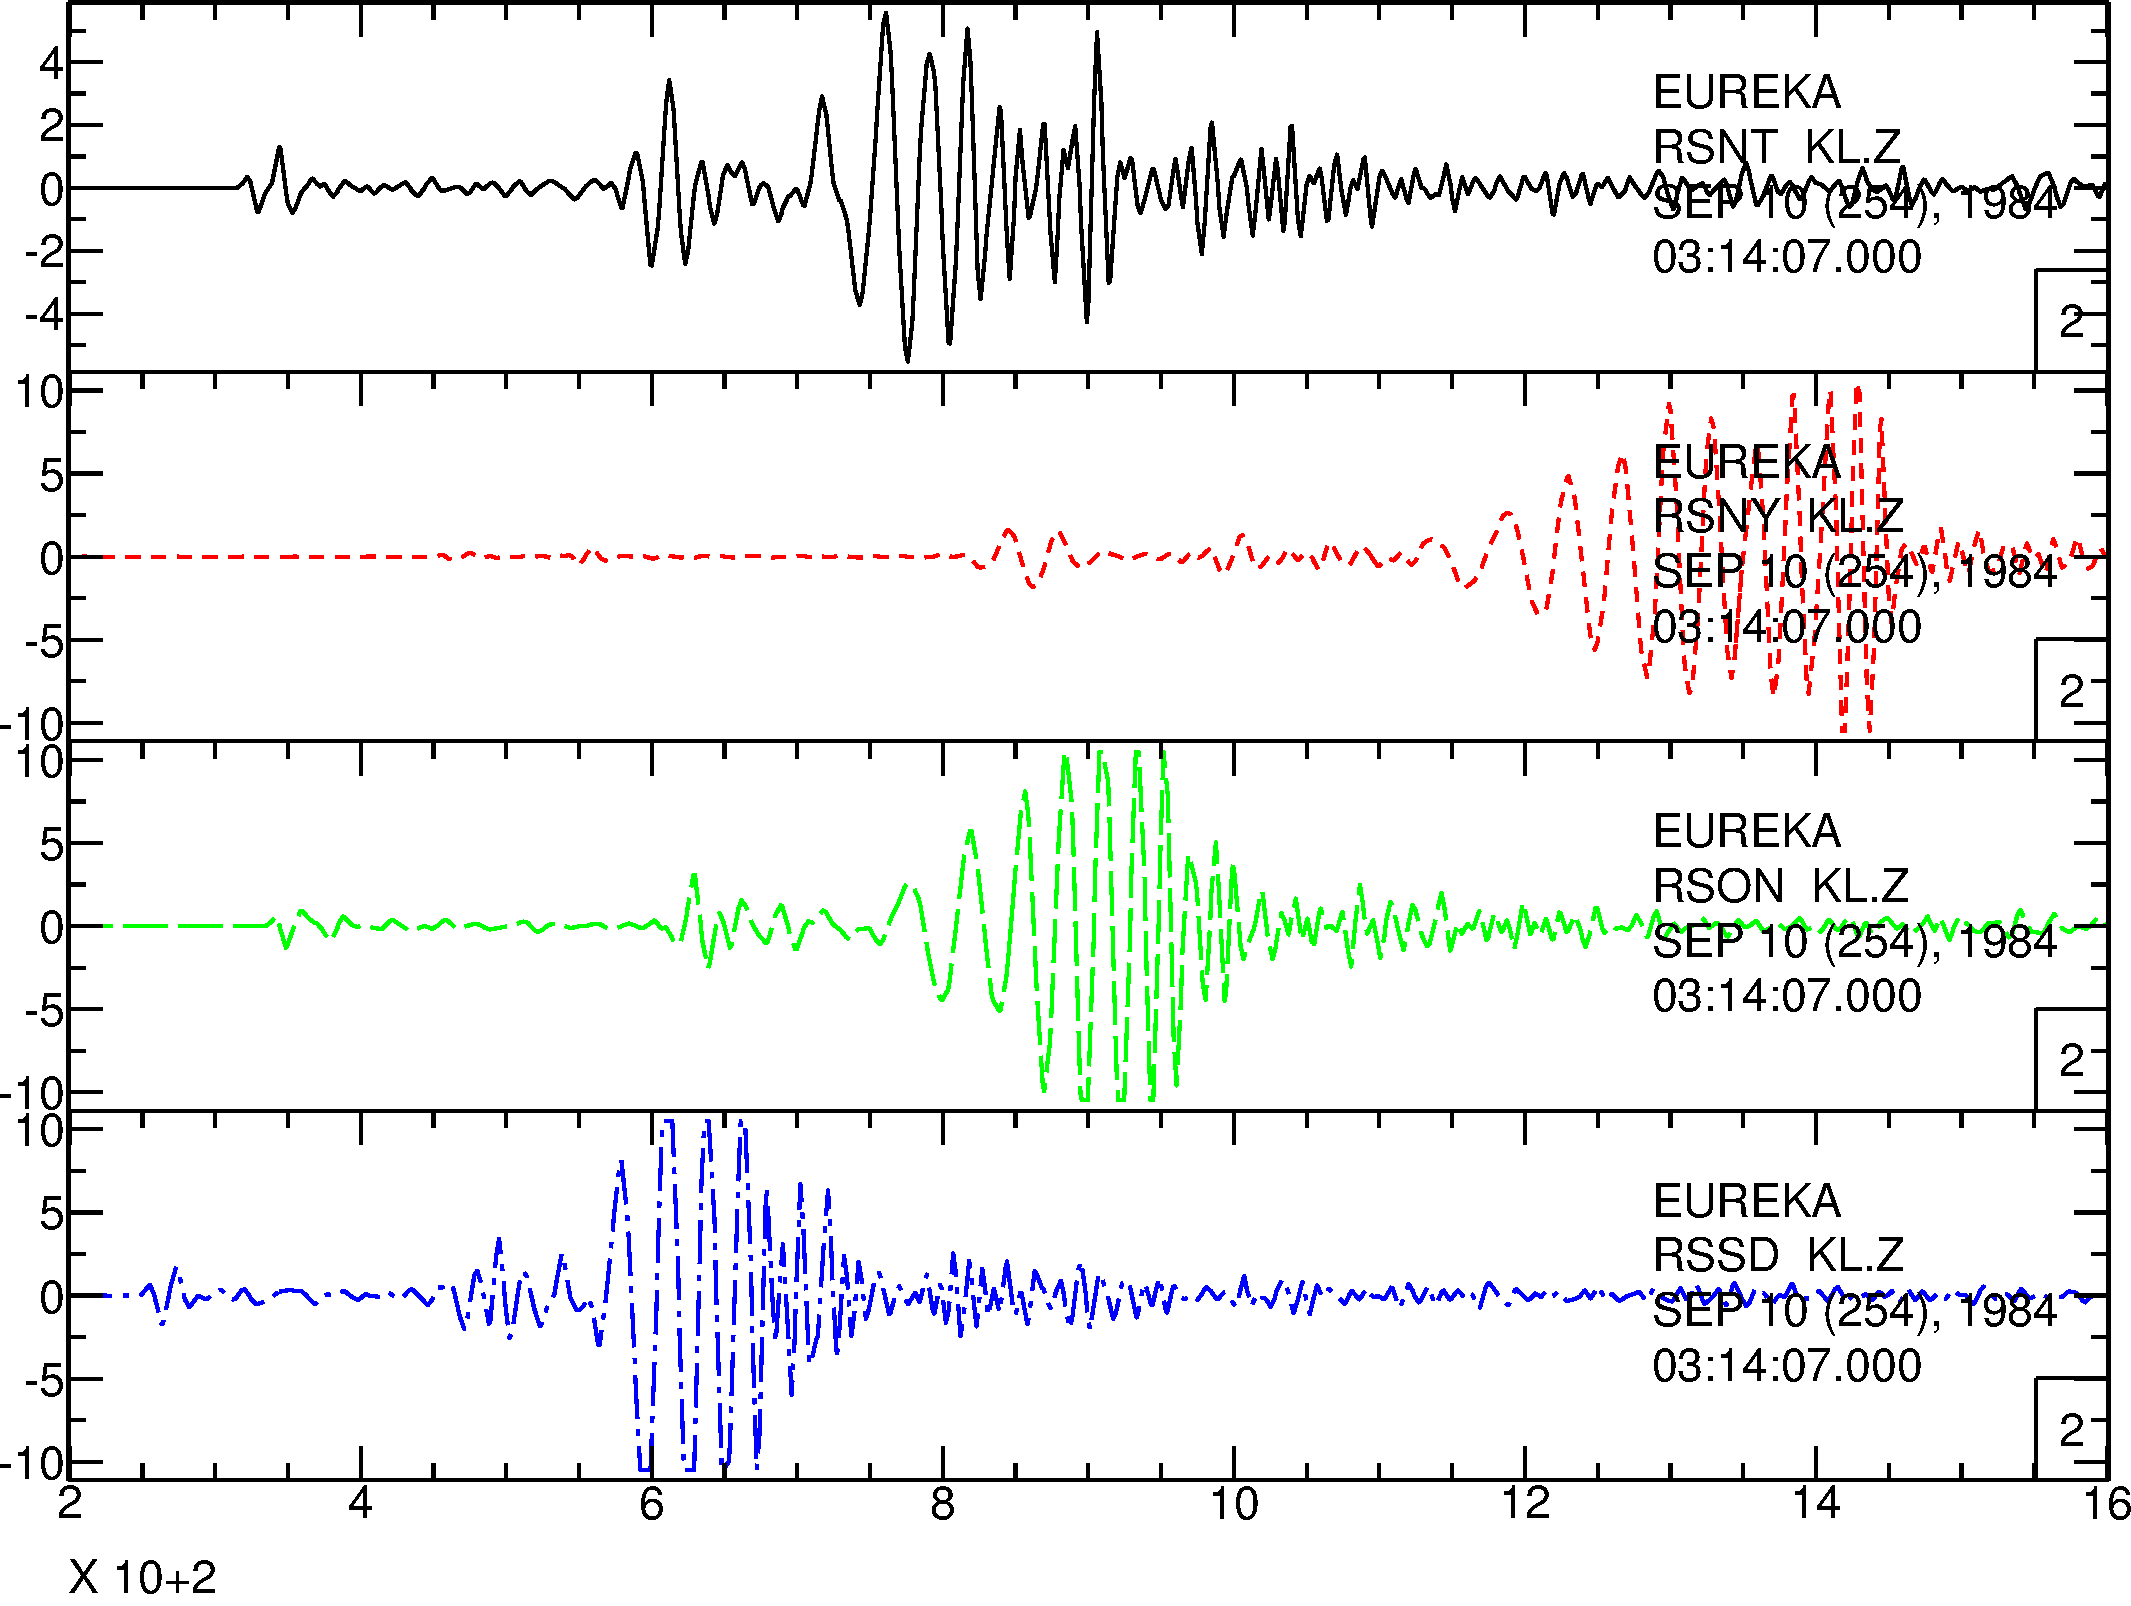
\includegraphics[width=0.7\textwidth]{attribution2}
\caption{线条属性递增}
\end{figure}

\nameref{cmd:line} 命令不仅可以设置线条的线型,同时可以对波形数据
进行颜色填充:
\begin{SACCode}
SAC> fg seis
SAC> qdp off
SAC> rmean; rtr; taper
SAC> line 0 fill red/blue
SAC> p
\end{SACCode}

\begin{figure}[H]
\centering
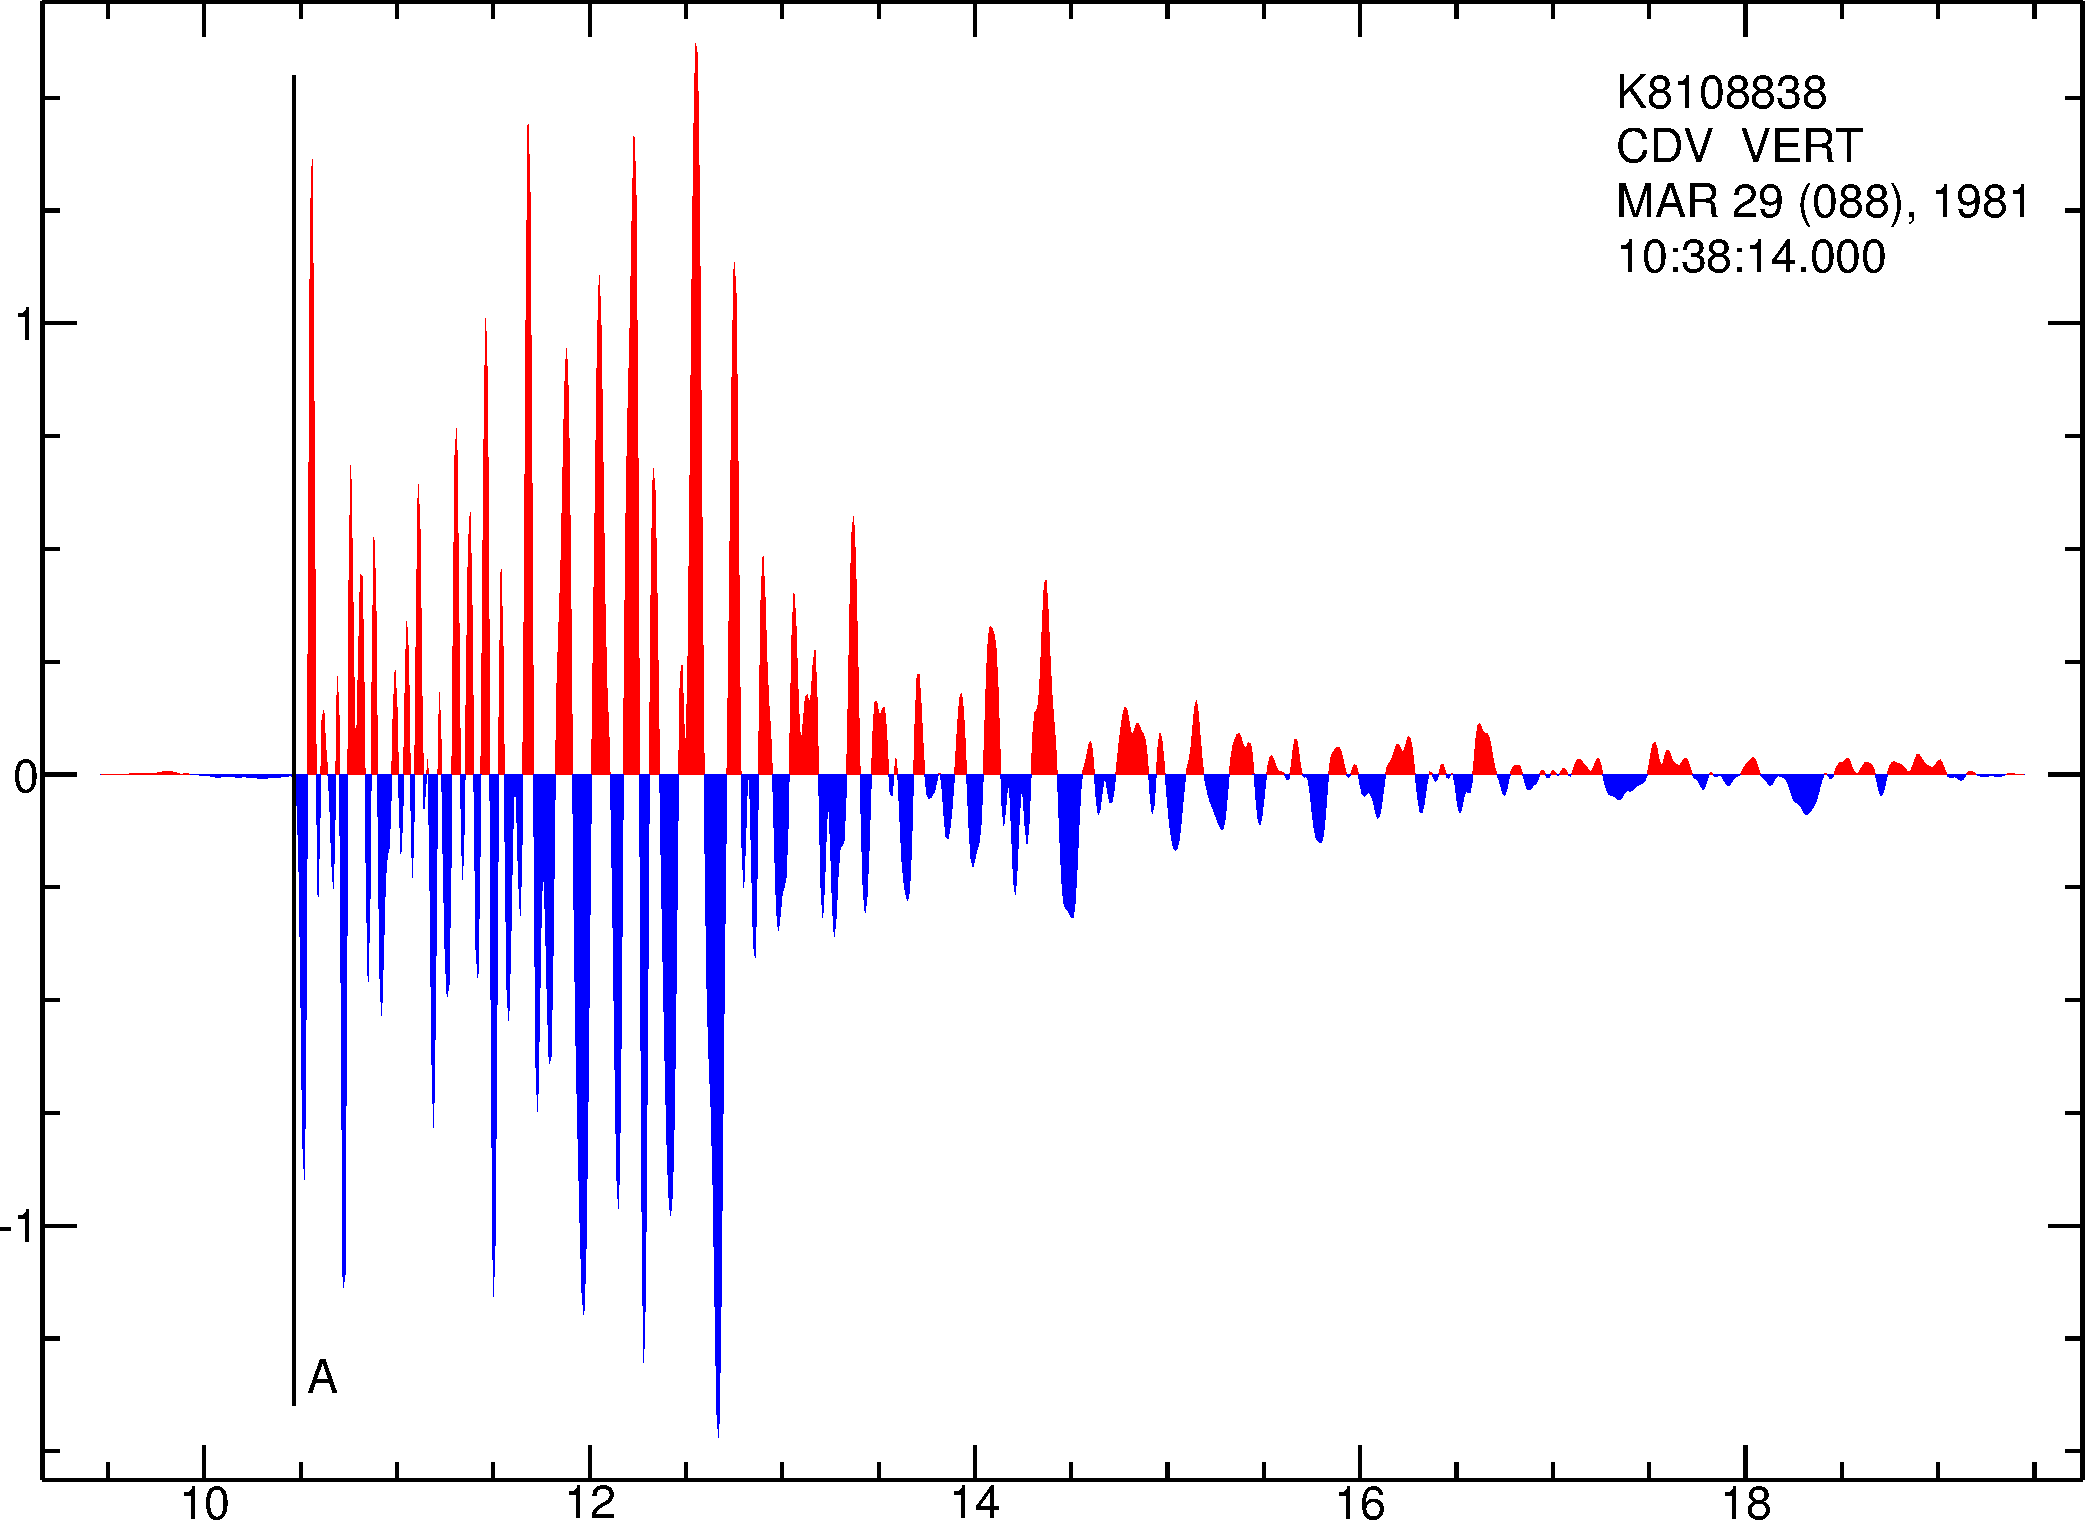
\includegraphics[width=0.7\textwidth]{linefill}
\caption{颜色填充图}
\end{figure}
